\documentclass[12pt]{article}
\usepackage[french]{babel}
\usepackage[utf8]{inputenc}
\usepackage{lmodern}
\usepackage[T1]{fontenc}
\usepackage{mathtools, amssymb, amsthm, amsmath, amsfonts}
\usepackage{graphicx, hyperref, xcolor, soulutf8, enumitem}
\usepackage{fancyhdr, lastpage, lipsum, xspace}

\title{\Huge{TP LATEX}}
\author{\Large{Naïm ZAIRI, Lucas LESAGE et Maurin GILLES}}
\date{\Large{Janvier 2022}}

\hypersetup{colorlinks = true, linkcolor=black, urlcolor = blue}
\setlength{\headheight}{15pt}
\addtolength{\topmargin}{-0.5pt}

\newtheorem{theorem}{Théorème}[subsubsection]
\newtheorem{definition}{Définition}[subsubsection]
\newtheorem{corollary}{Corollaire}[subsubsection]
\newtheorem{lemma}{Lemme}[subsubsection]
\newtheorem{example}{Exemple}[subsubsection]
\newtheorem{history}{Histoire}[subsubsection]
\newtheorem{property}{Propriétés}[subsubsection]
\newcommand{\ens}[1]{\mathbb{#1}}
\newcommand{\red}[1]{\textcolor{red}{#1}}

\pagestyle{fancy}
\lhead{Naïm ZAIRI, Lucas LESAGE et Maurin GILLES}
\rhead{Janvier 2022}
\cfoot{Page \thepage \ sur \pageref{LastPage}}

\frenchbsetup{StandardLists=true}



%%%%%%%%%%%%%%%% PRELIMINAIRES %%%%%%%%%%%%%%%%



\begin{document}


\maketitle 

\tableofcontents



%%%%%%%%%%%%%%%% FIN INTRODUCTION %%%%%%%%%%%%%%%%



\newpage
\part{L'arithmétique}
\setcounter{section}{0}

\section{L'ensemble des entiers naturels}

\subsection{Notation}

Comme leur nom l'indique, les entiers dits "naturels" correspondent aux nombres tels qu'on se les représente de manière naturelle.
Concrètement, ce sont ceux qui nous permettent de compter dans la vie de tous les jours.

D'un point de vue mathématique, on peut définir les entiers naturels comme les nombres strictement positifs qui peuvent s'écrire sans virgule.\\
\\

L'infinité de cet ensemble est intuitive. En effet, en partant de 0, et en comptant de 1 en 1, il apparait évident qu'on pourra toujours rajouter 1, et que le comptage n'aura jamais de fin.

L'infinité de l'ensemble nous oblige donc à avoir recours à une notation spéciale pour le désigner. La notation que nous utilisons encore aujourd'hui nous vient de \textit{Richard Dedekind}\ref{itm:entnat}. Il s'agit d'un N capital, stylisé de la manière suivante : 
$\ens{N}$

\subsection{Quelques propriétés intéressantes}
\subsubsection{Comparaison avec les autres ensembles usuels}

De par sa définition, l'ensemble $\ens{N}$ est le plus évident, mais donc aussi le plus basique des ensembles. Quand les mathématiques se sont complexifiées, d'autres ensembles ont été définis.

L'ensemble des entiers relatifs, noté $\ens{Z}$, comprend l'ensemble $\ens{N}$, auquel s'ajoutent tous les entiers négatifs.

L'ensemble des décimaux, noté $\ens{D}$, comprend tous les nombres pouvant s'écrire sous la forme $\frac{a}{10^b}, \text{avec} \ a \in \ens{Z} \ \text{et} \ b \in \ens{N}$.
Concrètement, on retrouve l'ensemble $\ens{Z}$ pour $b = 0$. 

L'ensemble des rationnels, noté $\ens{Q}$, comprend tous les nombres pouvant s'écrire sous la forme d'une fraction. Autrement dit, il s'agit de tous les nombres qui s'écrivent sous la forme $\frac{a}{b}, \text{avec} \ a \in \ens{Z} \ \text{et} \ b \in \ens{N}$.

L'ensemble des réels, noté $\ens{R}$, comprend l'ensemble des nombres qui peuvent s'écrire avec simplement une partie entière et une liste, potentiellement infinie, de décimales. Cela comprend l'ensemble $\ens{Q}$, ainsi que des nombres tels que $e$ ou $\pi$.\\
\\


Comme nous avons pu le voir, ces ensembles peuvent être vus comme plus ou moins grands, dans la mesure ou certains ensembles sont strictement compris dans d'autres.

En notation mathématique, on peut écrire : 
$\ens{N} \subset \ens{Z} \subset \ens{D} \subset \ens{Q} \subset \ens{R}$

On peut aussi se représenter les choses de façon plus visuelle avec un schéma de ce type (voir figure \ref{fig:schm_ensembles}).

\begin{figure}[h]
    \centering
    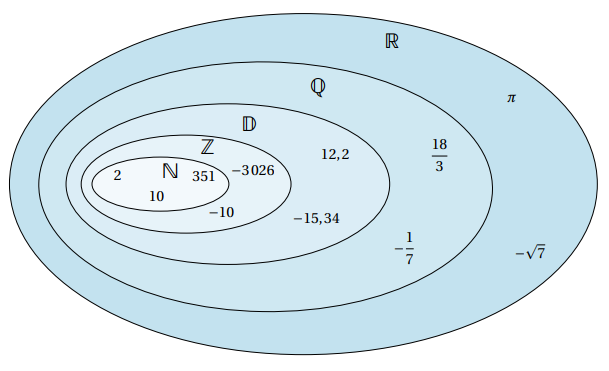
\includegraphics[scale=0.5]{schema_ensembles.png}
    \caption{Schéma Ensembles}
    \label{fig:schm_ensembles}
\end{figure}

(Note : si l'on s'aventure du côté des structures algébrique, on peut remarquer que l'ensemble $\ens{N}$ est le seul ensemble des cinq à ne pas être un groupe\ref{itm:Groupe})

\subsubsection{Infinis dénombrables}

Par son aspect intuitif pour compter, on utilise souvent l'ensemble $\ens{N}$ pour étudier la cardinalité d'un autre ensemble.

\begin{definition}
\textbf{Cardinalité :} \newline
La cardinalité d'un ensemble $E$, notée $card(E)$, correspond au nombre d'élements de $E$.
\end{definition}

\begin{corollary}
\textbf{Ensembles finis} : \newline
$E$ est un ensemble fini si et seulement si $card(E) \in \ens{N}$ .
\end{corollary}

Plus rigoureusement, dire que $card(E)=n$ veut dire que l'on peut faire une bijection\ref{itm:Bijec} entre l'ensemble $E$ et l'ensemble $\{1, \ldots ,n\} \subset \ens{N}$. \newline
\newline
Maintenant que nous avons traité le cas des ensembles finis, regardons quand ces ensembles sont infinis : \newline
\newline
Premièrement, on remarque que l'infini peut contenir l'infini... et peut aussi être contenu dans un autre infini ! ($2\ens{N} \subset \ens{N} \subset \ens{Z}$) \newline
Compliqué de dégager une cardinalité précise de tout ça... \newline
Mais de ce problème s'ensuit une définition fondamentale sur la cardinalité :

\begin{definition}
\textbf{Infinis dénombrables} : \newline
Soit $E$ un enemble infini. S'il existe une bijection entre $E$ et $\ens{N}$, alors on dit que $E$ est un ensemble dénombrable.
On note sa cardinalité par ce signe :
$$Card(\ens{N}) = \aleph_0$$
\end{definition}

Maintenant, avec cette définition, nous avons une réponse pour les cardinalités infinies. \newline
Regardons lesquels des ensembles usuels sont dénombrables :

\begin{theorem}
\label{thm:CrdEnU}
\textbf{Cardinalités des ensembles usuels} : \newline
$$Card(\ens{N})=Card(\ens{Z})=Card(\ens{D})=Card(\ens{Q})$$
\end{theorem}

\begin{proof}
La démonstration étant longue et hors-sujet, elle est donc libre à vous de la trouver par vous même ou d'aller chercher la réponse sur internet !
\end{proof}

Aussi fou que cela puisse paraître, même des ensembles qui paraissent intuitivement bien plus grands possèdent finalement la même cardinalité que $\ens{N}$. \newline
Mais dans le théorème \ref{thm:CrdEnU}, on voit que l'ensemble des Réels manque à l'appel !

\begin{theorem}
\textbf{Infinis indénombrables} : \newline
Il  n'existe aucune bijection entre l'ensemble $\ens{N}$ et l'ensemble $\ens{R}$. \newline
Par conséquent,
\begin{align*}
    Card(\ens{R}) & \not= \aleph_0 \\
    & = c \ \text{("continu")}
\end{align*}

Par définition :
$$2^{\aleph_0} = c$$
\end{theorem}

\begin{proof}
Voir la diagonale de G. Cantor \ref{itm;DiaCan}.
\end{proof}


Et bien finalement si, certains ensembles infinis sont vraiment plus grands que... l'infini. \newline
\newline
Une autre question se pose donc : combien y a-t-il d'infinis ? \newline
Et bien pour l'instant nous n'avons pas encore de réponse. La possible existence d'un cardinal compris entre $\aleph^{0}$ et $\aleph^{1}$ s'appelle \textit{"L'hypothèse du continu"}\ref{itm:HyDuCo}.
\newline
\newline
Conclusion : cet ensemble des plus simples est un puissant outil dans l'analyse des cardinaux.

\section{L'arithmétique de Peano}
\subsection{Introduction à l'arithmétique}

À l'époque de la Grèce Antique, les nombres en mathématique ne se limitaient qu'aux entiers naturels. \newline
En effet, même les nombres décimaux étaient représentés sous forme d'entier en changeant  la base. \newline
Par exemple : si une longueur géométrique mesurait $1,9 m$ alors à la place on disait que la longueur mesurait $19 dm$ et on adaptait ainsi toutes les autres mesures. \newline
\newline
(Anecdote : c'est par cette logique qu'un Pythagoricien a démontré l'existence de nombres irrationnels, des nombres ne pouvant pas être ramenés à une base car possédant une infinité de chiffres derrière la virgule \ !) \newline

Par conséquent, les opérations élementaires de l'arithmétique étaient l'addition, la soustraction, la multiplication et la division. \newline
Alors que l'addition et la multiplication sont des opérations triviales conservant la qualité d'entier d'un nombre, pour la division c'est une autre paire de manche (concernant la soustraction, l'introduction des entiers relatifs réglera ce problème). \newline
La division classique était appelée à l'époque "Division Euclidienne". \newline
Créée par le mathématicien Grec \textit{Euclide}\ref{itm:Euclide}, cette division, bien que réadaptée au fil du temps pour s'appliquer aux entiers relatifs,  permettait de ne pas avoir de partie fractionelle car il définissait une division comme étant un quotient et un reste.

\begin{theorem}
\textbf{Division Euclidienne} (Version adaptée) : \newline
Soient $a \in \ens{Z}$ et $b \in \ens{N}$, alors $\exists! (q,r) \in \ens{Z} \times \ens{N}$ avec $0 \leq r < b$ tels que : \newline
$$a = bq + r$$
\end{theorem}

(Note : la démonstration étant assez longue et hors-sujet, nous vous laissons voir la référence \ref{itm:DivEuc}) \newline

Cette définition de la division euclidienne peut sembler quelque peu abrupte, mais en fait cela est équivalent à la division euclidienne que l'on faisait en primaire ! (voir figure \ref{fig:DivEuc}) \newline

a := Dividende / b := Diviseur / q := Quotient / r := Reste
\begin{figure}[h]
    \centering
    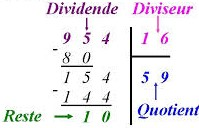
\includegraphics{division_euclidienne.jpg}
    \caption{Division euclidienne}
    \label{fig:DivEuc}
\end{figure}
\newline \newline \newline
Au cours du temps l'arithmétique n'a fait que se complexifier et se mélanger avec d'autres disciplines et créer d'autres types d'arithmétiques :

\begin{itemize}
    \item l'arithmétique modulaire \ref{itm:AriMod}
    \item la théorie algébrique des nombres \ref{itm:AriAlg}
    \item l'arithmétique des polynômes \ref{itm:AriPol}
\end{itemize}

Mais, pendant la crise des fondements\ref{itm:CriFon}, le mathématicien italien \textit{Giuseppe Peano}\ref{itm:Peano} décida en 1889 de formaliser l'arithmétique en créant un système axiomatique que l'on appela "l'arithmétique de Peano". \newline
C'est le début des fondations de l'arithmétique moderne, mais, avant de s'atteler à cette arithmétique, nous devons d'abord introduire les symboles de la logique mathématique.

\subsection{Introduction aux symboles}

Un théorème de l'arithmétique de Peano est forcément écrit par ces symboles :

\paragraph{Opérateurs et inconnues}
\textbf{:} \newline
Les 2 opérateurs : $+ \ \times$ \newline
Des lettres, que ce soit, latines, grecques, parfois avec des indexations, majuscules ou minuscules : $x$, $y$, $\delta$, $x_n$ \ldots

\paragraph{Quantificateurs :}
Les 2 uniques quantificateurs et leur variation : \newline
$\forall$ : Pour tout / Quel que soit \newline
$\exists$ : Il existe \newline
$\exists!$ : Il existe un unique 

\paragraph{symboles logiques :}
Les symboles de la logique classique : \newline
$\implies$ : implication \newline
$\Longleftrightarrow$ : équivalence \newline
$\wedge$ : et \newline
$\vee$ : ou \newline
$\neg$ : négation \newline
$=$ : égalité \newline
$P(x, \ldots ,x_n)$ : Une propriété dépendant de $n$ variables \newline

\paragraph{symboles de Peano :}
Alors que les opérateurs, les quantificateurs et les symboles logiques peuvent être trouvés dans d'autres théories, les 2 prochains symboles sont propres à l'arithmétique de Peano : \newline \newline
1) la constante $0$ : seul chiffre pouvant être écrit car son existence est assumée par l'ensemble axiomatique de Peano (nous traiterons plus profondément de ce sujet dans la section \ref{sec:AxioPea}). \newline \newline
2)La fonction $S$ (Successeur). \newline
On pourrait intuitivement la définir comme :
\begin{align*}
    S : \ & \ens{N} \ \to \ \ens{N} \\
        & n \ \mapsto \ n+1 \\
\end{align*}
(Note : il faut bien comprendre qu'ici la fonction est une idée, il ne faut pas l'imaginer dans le sens d'une fonction à proprement parler. Nous l'avons mise sous cette forme pour aider à l'intuition mais à ce stade de la théorie, une fonction n'est même pas définie, c'est donc un non-sens de définir un axiome sur quelque chose qui n'existe pas.)


\subsection{Les axiomes de l'arithmétique de Peano}
\subsubsection{Définition d'un axiome et d'un système axiomatique}

Avant de se lancer à bras le corps dans le système axiomatique de Peano, il est important d'avoir une compréhension complète de ce que sont un axiome et un système axiomatique. \newline

\begin{definition} \label{def:Axiome}
\textbf{Axiome} \ref{itm:Axiome} : \newline
Proposition considérée comme évidente, admise sans démonstration.
\end{definition}
\begin{definition} \label{def:SysAxi}
\textbf{Système axiomatique} \ref{itm:SysAxi} : \newline
Ensemble d'axiomes dont certains ou tous les axiomes peuvent être utilisés logiquement pour dériver des théorèmes.
\end{definition}

Analysons plus en détail leur signification : \newline
Premièrement, avant de comprendre la définition, il est important de comprendre la motivation d'une telle définition. \newline
Si l'on devait faire une analogie, l'ensemble des théories mathématiques équivaudrait à un arbre. Chaque branche est un théorème et chaque feuille ou branche liée à cette dernière est un corrolaire ou un nouveau théorème. \newline
En effet, chaque théorème utilise des informations issues d'un autre théorème prouvé préalablement (et parfois même pas prouvé d'ailleurs...!) et ainsi de suite. \newline
Par conséquent, les axiomes sont les racines de cet arbre, les "théorèmes originaux". \newline
C'est pourquoi, d'après la définition \ref{def:Axiome}, les axiomes sont des propositions, car s'il existait une démonstration, ils seraient des théorèmes et non des axiomes. \newline
\newline
Ainsi, avec plusieurs axiomes on forme un système axiomatique, et c'est en combinant ces axiomes de manière logique qu'on peut ainsi créer des théorèmes, et ainsi de suite. \newline
Un système axiomatique est la base d'une théorie (exemple : la théorie des ensembles ZFC (\ref{itm:ThrZFC}) ou l'arithmétique de Peano). Ils diffèrent selon les théories, qui sont parfois plus ou moins complètes (on les appelle des théories de premier ordre (\ref{itm:CalPre}) par exemple). \newline
Le plus important pour une théorie est que'elle soit cohérente (même si on ne peut pas prouver qu'elle l'est ou non (\ref{itm:ThmGdl}) !).

\begin{definition}
\textbf{cohérence} : \newline
La cohérence est la propriété d'une théorie exempte de contradiction.
\end{definition}

Plus intuitivement, un système axiomatique est dit incohérent s'il est possible de former 2 théorèmes qui prouvent quelque chose et son contraire. \newline
Pour bien comprendre le principe d'un système axiomatique, regardons un petit exemple :

\begin{example}
Créons une théorie : \newline
Axiome 1 : les mammifères ne pondent pas des œufs. \newline
Axiome 2 : les ornithorynques sont des mammifères. \newline
Axiome 3 : les ornithorynques pondent des œufs. \newline

Nous venons de créer un système axiomatique avec ces 3 axiomes, regardons les théorèmes que l'on peut faire avec : \newline
\newline
Théorème : les ornythorinques ne sont pas des mammifères (axiome 1+3). \newline
\newline
Une contradiction !! Nous venons de créer un théorème qui contredit notre axiome 2. Par conséquent notre théorie est incohérente et n'est donc pas valide.
\end{example}

Maintenant que nous avons mis au clair une définition précise des axiomes et des systèmes d'axiomatiques, rentrons dans le cœur du sujet.


\subsubsection{Le système axiomatique de l'arithmétique de Peano}
\label{sec:AxioPea}
L'arithmétique de Peano repose entièrement sur ces 5 axiomes :

\begin{enumerate}
    \item L'élément appelé \textit{zéro} et noté $0$ est un entier naturel.
    \item Tout entier naturel $n$ a un unique successeur, noté $s(n)$ ou $Sn$ qui est un entier naturel.
    \item Aucun entier naturel n'a $0$ pour successeur.
    \item Deux entiers naturels ayant le même successeur sont égaux.
    \item Si un ensemble d'entiers naturels contient $0$ et contient le successeur de chacun de ses éléments, alors cet ensemble est $\ens{N}$ (on appelle plus communément cette propriété "la récurrence").
\end{enumerate}

\textbf{Il est important de comprendre que ces 5 axiomes ne définissent non pas l'arithmétique de Peano, mais l'ensemble des entiers naturels $\ens{N}$.} \newline
\newline
De manière plus intuitive, cette définition axiomatique définit $\ens{N}$ comme un ensemble : \newline
1) Non-vide (car il contient l'élément $0$). \newline
2) Infini (car chaque élément possède un successeur). \newline
3) Comprenant des entiers uniquement positifs (car pour que $0$ soit le successeur d'un nombre $n$ alors il faudrait, par définition de $S(n)$, que $n=-1$). \newline
4) Ordonné (chaque élément ayant un unique successeur et inversement, on peut ainsi comparer les entiers entre eux, exemple : $3 < 4$). \newline
\newline
(Note : le $5^{\text{ème}}$ axiome pose la définition que cet ensemble est bien équivalent à l'ensemble $\ens{N}$) \newline

Maintenant que les bases de l'ensemble $\ens{N}$ ont été posées et que nous avons introduit les symboles de la logique, introduisons les 8 axiomes du système axiomatique de l'arithmétique de Peano :

\begin{enumerate}
    \item $\forall x \ \neg(S(x)=0)$ \newline
    (Il n'existe aucun élément $x$ tel que son successeur est égal à $0$)
    
    \item $\forall x \ (x=0 \vee \exists y (x=S(y)))$ \newline
    (Quel que soit l'élément $x$, soit il est égal à $0$, soit il est le successeur d'un autre élément)
    
    \item $\forall x \forall y \ (S(x)=S(y) \implies x=y)$ \newline
    (Si 2 éléments ont le même successeur alors ils sont égaux)
    
    \item $\forall x \ (x+0=x)$ \newline
    ($0$ est l'élement neutre de l'addition)
    
    \item $\forall x \forall y \ (x+S(y) = S(x+y))$ \newline
    (Se traduit intuitivement : $x + (y + 1) = (x + y) + 1$)
    
    \item $\forall x \ (x \times 0 = 0)$ \newline
    ($0$ est l'élement absorbant de la multiplication)
    
    \item $\forall x \forall y \ (x \times S(y) = (x \times y) + x)$ \newline
    (Se traduit intuitivement : $x \times (y+1) = (x\times y) + x$, par distributivité)
    
    \item $\forall F(x, x_1, \ldots , x_n)$, $\forall x_1 \ldots \forall x_n$  : \newline
    $((F(0,x_1,\ldots,x_n) \wedge (\forall x (F(x,x_1,\ldots,x_n) \implies F(S(x),x_1,\ldots,x_n)))) $ \newline 
    $\implies \forall x F(x,x_1,\ldots,x_n)$
\end{enumerate}

Bon, vous n'avez peut-être rien compris à l'axiome 8... et c'est bien normal ! Le coup de génie de Peano ici est de, même avec un langage simple, généraliser la récurrence à n'importe quel type d'affirmation (ici appélée $F$). Disséquons cet axiome : \newline
\newline
Premièrement, enlevons tout les $x_1, \ldots, x_n$. On obtient donc, \newline
$$(F(0) \wedge (\forall x (F(x) \implies F(S(x)))) \implies \forall x F(x)$$ \newline
Sous cette forme on peut reconnaître le principe de récurrence, si on traduisait l'expression littéralement on aurait : \newline
\textit{Si une affirmation est vraie pour $0$, et si le fait qu'elle soit vraie pour $x$ implique qu'elle soit vraie pour $x+1$, alors l'affirmation est vraie pour tout élément $x \in \ens{N}$.} \newline
\newline
Maintenant que nous avons compris la structure de l'axiome, il est temps de le généraliser. \newline
En rajoutant tous ces $x_1, \ldots ,x_n$, alors on généralise une affirmation à n'importe quelle affirmation existante. \newline
\textbf{Peu importe l'affirmation $F$ et peu importe le nombre de paramètres de cette fonction, tant qu'elle possède une notion d'hérédité sur un de ses éléments alors il y a récurrence.}


\subsection{Conclusion}
L'arithmétique est une discipline millénaire, originellement due à nos connaissances des nombres limitée, mais finalement élargie et complexifiée par le temps, devenant un outil très utilisé en cryptographie, par exemple. \newline
C'est aussi à la fois une discipline très ardue et souvent très abstraite. Cela nous fait comprendre que la base même des nombres, les plus simples, les plus intuitifs, renferment énormément de secrets et de connaissances qu'il nous tarde de découvrir. \newline
\newline
\textit{"La mathématique est la reine des sciences et l’arithmétique est la reine des mathématiques"}
\begin{flushright}
-C. F. Gauss
\end{flushright}



%%%%%%%%%%%%%%%% FIN PARTIE 1 %%%%%%%%%%%%%%%%



\newpage
\part{Les nombres premiers}
\setcounter{section}{0}
\section{Définition et histoire}
\begin{definition}
\label{def:nb_prem}
Un entier n supérieur ou égal à deux est dit premier si et seulement si ses seuls diviseurs positifs sont 1 et lui-même.
\end{definition}

\begin{theorem} \label{thm:InfPre}
Il y a une infinité de nombres premiers.
\end{theorem}


\begin{proof}
Nous allons maintenant démontrer par l'absurde qu'il existe une infinité de nombres premiers. \\
Supposons que P soit fini, de cardinal n. Soient $p_1,...,p_n$ ses éléments. \\
Posons $N= 1 + p_1 ... p_n$. On a $N \geq 2$, donc N possède un diviseur premier p (d'apres \ref{itm:divprem}). \\
L'entier p divise $p_1 ... p_n$, d'où l'on déduit que p divise 1. Cela conduit à une contradiction. P est donc infini.
\end{proof}

\begin{history} \ref{histoire}
On peut retrouver des traces des nombres premier à 20 000 ans avant notre ère, sur l'os d'Ishango où figurent les nombres 11, 13, 17 et 19. \\
Durant l'antiquité, Euclide met en place des théories et des affirmations dans les "Eléments", ainsi que la décomposition en facteurs premiers. Puis, ce sera Eratosthène de Cyrène qui donnera une méthode simple pour déterminer les nombres premiers. \\
Par la suite, au Moyen-Age, ce sera Fibonnacci qui en fera une liste et en déterminera des critères de divisibilité. Ce sera un ecclésiastique français du nom de Marin Mersenne qui posa la question : si p est premier est-ce que $2^p - 1$ est premier ? Il a été montré que non, cependant la méthode est encore utilisée pour déterminer les nombres premiers dits "géants". \\
Ce sera ensuite durant la Renaissance que Goldbach affirmera que tout nombre peut s'écrire sous forme d'une somme de deux nombres premiers. Euler quant à lui prouvera que $2^{31} - 1$ est premier. Gauss et Legendre vont par la suite s'intéresser à la repartition des nombres premier, montrant que plus les nombres sont dits "géants", moins les nombres premiers seront présents. \\
Aujourd'hui, le plus grand nombre premier connu a été decouvert en 2018 et est : $2^{82 \ 589 \ 933} - 1$.
\end{history}


\section{Le théorème fondamental de l'arithmétique}

Concernant les nombres premiers, les deux théorèmes à la fois les plus importants et les plus anciens, sont : \newline
-Il y a une infinité de nombres premiers (Théorème \ref{thm:InfPre}). \newline
-Le théorème fondamental de l'arithmétique.

\begin{theorem}
\textbf{Théorème fondamental de l'arithmétique} : \newline
Tout entier $n > 0$ peut être écrit comme un produit de nombres premiers, de façon unique.
\end{theorem}

De ce théorème s'ensuivent un corollaire et une définition :

\begin{corollary}
\textbf{Nombres premiers} : \newline
Un nombre est premier si et seulement si il est l'unique facteur de sa décomposition.
\end{corollary}

\begin{definition}
\textbf{Nombres composés} : \newline
Un entier $n > 0$ est dit composé si et seulement si il est le produit d'au moins $2$ nombres.
\end{definition}

Regardons quelques exemples pour bien comprendre comment marche une décomposition : 

\begin{example}
: \newline
- $6 \ 936 = 2^{3} \times 3 \times 17^{2}$ \newline
- $1 \ 200 = 2^{4} \times 3 \times 5^{2}$ \newline
- $7 = 7$ \newline
Les deux premiers nombres sont donc des nombres composés tandis que le dernier nombre est premier.
\end{example}

(La manière dont on trouve ces décompositions sera vue plus en profondeur dans les sections \ref{sec:algo_euclide} et \ref{sec:Algorithme})


\subsection{démonstration}

Pour démontrer le Théorème fondamental de l'arithmétique, il est nécessaire de le diviser en 2 parties. \newline
En effet, le théorème affirme l'existence d'une décomposition ; et l'unicité de cette dernière. \newline
Il nous faudra donc prouver son existence, et ensuite prouver que cette décomposition est unique. \newline
(La démonstration est issue d'une vidéo youtube \ref{itm:FunAri})

\subsubsection{Partie 1 : existence de la décomposition}

\begin{proof}
Nous ferons une démonstration par l'absurde : \newline
Supposons qu'il existe au moins un entier naturel qui ne possède \textbf{pas} une telle décomposition.\newline
On pose $m$, le plus petit de ces entiers. \newline
On observe que $m$ est forcément composé (sinon il serait premier et, par définition, serait sa propre décomposition). \newline
\newline
On pose donc, \newline
$$ m = ab \ \ \ \ \text{avec} \ 1 < a,b < m$$ 
Vu que $a,b < m$, on peut écrire $a$ et $b$ dans leur décomposition (car on a posé m comme étant \textbf{le plus petit} entier qui ne peut pas s'écrire sous cette forme). \newline
Donc :

\begin{equation*} \label{equ:a}
    a = p_1^{\alpha_1} \ldots p_n^{\alpha_n} \ \ \ \ p_i \ premiers \ / \ \alpha_i \in \ens{N} \ \ (1 \leq i \leq n)
\end{equation*}
\begin{equation*} \label{equ:b}
    b = q_1^{\beta_1} \ldots q_m^{\beta_m} \ \ \ \ q_i \ premiers \ / \ \beta_i \in \ens{N} \ \ (1 \leq i \leq m)
\end{equation*}
\newline
mais par définition de $m$, on a :
\begin{align*}
    m & = ab \\
      & = p_1^{\alpha_1} \ldots p_n^{\alpha_n} \times q_1^{\beta_1} \ldots q_m^{\beta_m} \\
\end{align*}
$m$ possède donc une décomposition en facteurs premiers, ce qui contredit le prédicat. \newline
Par conséquent, on conclut qu'il n'existe pas d'entier naturel $m$ qui ne possède pas de décomposition en facteurs premiers.
\end{proof}

\subsubsection{Partie 2 : unicité de la décomposition}

Avant de s'attaquer à l'unicité, nous devons d'abord introduire le lemme d'Euclide :

\begin{lemma}
\textbf{Lemme d'Euclide} : \newline
Soient $b,c \in \ens{N}$. \newline
Si un nombre premier $p$ divise le produit $b \times c$, alors $p$ divise $b$ \textbf{ou} $p$ divise $c$.
\end{lemma}

\begin{proof}
Voir la référence \ref{itm:LemEuc}.
\end{proof}

Maintenant que cela a été posé, commençons la démonstration de l'unicité de la décomposition en facteurs premiers :

\begin{proof}
Nous ferons aussi une démonstration par l'absurde : \newline
Supposons que $2$ décompositions différentes sont égales :
\begin{equation*}
    p_1^{\alpha_1} \ldots p_n^{\alpha_n} = q_1^{\beta_1} \ldots q_m^{\beta_m}
\end{equation*}
Nous avons 3 objectifs : \newline
1) Montrer que $n=m$. \newline
2) Montrer que $p_i=q_i \ \ (\forall i, \ 1 \leq i \leq n,m)$. \newline
3) Montrer que $\alpha_i=\beta_i \ \ (\forall i, \ 1 \leq i \leq n,m)$. \newline
\newline
Premièrement, on sait que :
$$p_i \ \text{divise} \ p_1^{\alpha_1} \ldots p_n^{\alpha_n} \ \ (\forall i, \ 1 \leq i \leq n)$$
mais par conséquent,
$$p_i \ \text{divise aussi} \ q_1^{\beta_1} \ldots q_m^{\beta_m} \ \ (\forall i, \ 1 \leq i \leq n)$$ 
(vu qu'ils sont censés être égaux) \newline

Mais si on applique plusieurs fois le lemme d'Euclide, on déduit que :
\begin{align*}
    & p_i \ \text{divise} \ q_r^{\beta_r} \ (\text{pour un certain} \ 1 \leq r \leq m) \\
    \implies & p_i \ \text{divise} \ q_r \\
\end{align*}
(Note : Si ces deux assertions ne vous paraissent pas évidentes, il faut comprendre que le lemme d'Euclide s'étend à autant de facteurs que vous le voulez. Vu que $p_i$ divise la décomposition de facteurs premiers, alors on sait que $p_i$ divise \textbf{au moins un} des facteurs, d'où la précision de "un \textbf{certain} $r$". \newline
Et vu que $p_i$ divise un nombre mis à une puissance, ce nombre n'a comme facteurs que lui même, d'où l'implication que $p_i$ divise $q_r$) \newline
\newline
Maintenant on sait que que $p_i$ divise $q_r$, mais on rappelle que $p$ et $q$ sont des nombres \textbf{premiers}.\newline
Par conséquent, ils ne possèdent aucun diviseur autre que 1 et eux-même, et vu que $p,q \not= 1$ (car $1$ n'est pas considéré comme premier), on conclut que :
$$p_i=q_r$$
Mais si l'on répète ce processus pour chaque facteur des deux côtés de l'égalité, alors on observe qu'à chaque facteur $p_i$ on peut associer un facteur $q_r$, et inversement. \newline
Par conséquent, on conclut que :
$$n=m$$
et que les deux décompositions possèdent les mêmes nombres premiers en facteurs. \newline
\newline
Maintenant que nous avons prouvé que les deux décompositions ont le même nombre de facteurs, et que ces facteurs sont égaux entre eux, il suffit de prouver que ces facteurs sont bien élevés aux mêmes puissances. \newline
Après avoir réarrangé les termes, on a :
\begin{equation} \label{equ:Facteurs}
    p_1^{\alpha_1} \ldots p_n^{\alpha_n} = p_1^{\beta_1} \ldots p_n^{\beta_n}
\end{equation}
On cherche donc à montrer que :
$$\alpha_i = \beta_i \ \ (\forall i, \ 1 \leq i \leq n)$$
\newline
Nous allons démontrer cela par l'absurde : \newline
Assumons que $\alpha_i > \beta_i$ \newline
Divisons les deux côtés de l'égalité (\ref{equ:Facteurs}) par $p_i^{\beta_i}$. On obtient donc l'égalité suivante :
\begin{equation} \label{equ:Division}
    p_1^{\alpha_1} \ldots p_i^{\alpha_i-\beta_i} \ldots p_n^{\alpha_n} = p_1^{\beta_1} \ldots p_{i-1}^{\beta_{i-1}} p_{i+1}^{\beta_{i+1}} p_n^{\beta_n}
\end{equation}
(Note : si vous n'avez pas bien compris, vu que $\alpha_i > \beta_i$, alors du côté gauche le facteur $p_i$ existe toujours, il a juste perdu en puissance, alors qu'à droite il a tout simplement disparu, emporté par la division.) \newline
\newline
Avec l'égalité (\ref{equ:Division}), on en déduit :
\begin{align*}
    & p_i \ \text{divise} \ p_1^{\alpha_1} \ldots p_i^{\alpha_i-\beta_i} \ldots p_n^{\alpha_n} \\
    \implies & p_i \ \text{divise} \ p_1^{\beta_1} \ldots p_{i-1}^{\beta_{i-1}} p_{i+1}^{\beta_{i+1}} p_n^{\beta_n} \\
    \implies & p_i \ \text{divise} \ p_j \ \ \ \text{avec} \ i \not= j 
    \ \ \ \text{\scriptsize{(D'après le lemme d'Euclide)}} \\
\end{align*}
Mais nous sommes face à une contradiction ! \newline
En effet, $p_i$ \textbf{ne peut pas} diviser $p_j$, car ces deux nombres ont été définis comme premiers. \newline
On en conclut donc que, $$\alpha_i \not> \beta_i$$ et avec la logique inverse on pourrait aussi prouver que, $$\alpha_i \not< \beta_i$$
\newline
Conclusion : $$\alpha_i = \beta_i \ \ (\forall i, \ 1 \leq i \leq n)$$
\newline
\newline
Nous avons démontré que si deux décompositions sont égales, alors cela implique qu'elles aient le même nombre de facteurs, que ces facteurs soient égaux entre eux, et que ces mêmes facteurs soient élevés à une même puissance. De cela nous pouvons enfin conclure que :
\begin{center}
    \textbf{La décomposition d'un nombre en facteurs premiers est unique.}
\end{center}

\end{proof}


\subsection{Forme générale d'une décomposition}
\label{sec:Decompo}

Maintenant que nous avons fini la démonstration, nous pouvons enfin énoncer le théorème :

\begin{theorem}
\textbf{Théorème fondamental de l'arithmétique} : \newline
$\forall n \in \ens{N} \backslash \{0,1\}$, $\exists! k \in \ens{N}^{*}$ avec $p_1 \ldots p_k$ des nombres premiers et \newline $\alpha_1, \ldots ,\alpha_k \in \ens{N}^{*}$ tel que :
$$n = p_1^{\alpha_1} \ldots p_k^{\alpha_k}$$
\end{theorem}

(Nous verrons des applications de ce théorème dans les sections \ref{part:pgcd_decompo} et \ref{part:ppcm_decompo})


\section{Deux outils de l'arithmétique}
\subsection{Le PGCD : Plus Grand Commun Diviseur}
\begin{definition} \normalfont
Soient a et b deux entiers dont au moins l'un des deux est non nul. On appelle \red{PGCD} le \red{P}lus \red{G}rand \red{C}ommun \red{D}iviseur de a et b. On note $a \bigwedge b$ le plus grand des diviseurs communs à a et b.
\end{definition}

\begin{property} \normalfont
Montrons quelques propriétés du PGCD : 
\begin{enumerate} \normalfont
\item $\forall a \in \mathbb{N}^*$, PGCD(a,0) = a et PGCD(a,1) = 1
\item PGCD(a,b) = PGCD (b,a)
\item \label{prop:homopgcd}
Si $ (a,b,k) \in \mathbb{Z}^3$, $(ka) \bigwedge (kb) = |k|(a \bigwedge b)$, cela représente l'homogénéité du PGCD. Soit PGCD(ka,kb) = k $\times$ PGCD(a,b)
\item Si b $\in \mathbb{N}^*$, et si a = bq + r est la division euclidienne de a par b, alors $a \bigwedge b = b \bigwedge r$
\item Pour tout couple $(a,b) \in \mathbb{Z}^2$, il existe $(u,v) \in \mathbb{Z}^2$ tel que : \\
$au + bv = a \bigwedge b$. Le couple (u,v) est appelé couple de coefficient de Bezout. \\
Si $au + bv = 1$, on peut déduire que a et b sont premiers entre eux, c'est à dire que a ne divise pas b, et reciproquement que b ne divise pas a.
(On appelle cette propriété : "Théorème de Bachet-Bézout"\ref{itm:ThmBaBe})
\end{enumerate}
\end{property}

\begin{example} \normalfont
Voici quelques exemples de PGCD:
\item PGCD(60,100) = 20
\item PGCD(252,360) = 36 
\item PGCD(2730,5610) = 30
\end{example}


\subsubsection{L'Algorithme d'Euclide} \normalfont
\label{sec:algo_euclide}

\begin{definition} \normalfont
L'Algorithme d'Euclide est un algorithme permettant de calculer facilement le PGCD de deux nombres a et b. Pour cela, il faut calculer la division euclidienne de a par b. Ensuite a prend la valeur de b et b prend la valeur du reste. On répète l'opération jusqu'à ce que b soit égal à 0. On prend alors la valeur (finale) de a. \newline
Pour mieux comprendre ce propos, en voici une illustration (Figure \ref{fig:euclide}) ainsi qu'un exemple.

\begin{example} \normalfont
PGCD(360, 252): \newline
$360 = 252 \times 1 + 108$ \newline
$252 = 108 \times 2 + 36$ \newline
$108 = 36 \times 3 + 0$ \newline
Le PGCD de 360 et 252 est 36.
\end{example}

\begin{figure}[h]
    \centering
    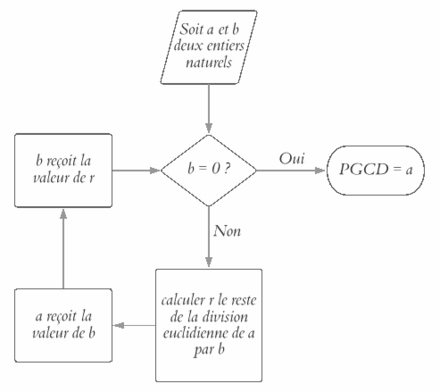
\includegraphics[scale=0.5]{algo.jpg}
    \caption{Algorithme Euclide}
    \label{fig:euclide}
\end{figure}

\end{definition}
\subsection{Le PPCM : Plus Petit Commun Multiple}
Le \red{PPCM} signifie \red{P}lus \red{P}etit \red{C}ommun \red{M}ultiple.

\begin{definition}
Soient a et b deux entiers. Les assertions suivantes sont équivalentes :
\begin{itemize}
    \item a est un multiple de b
    \item b est un diviseur de a
    \item b|a
    \item $\exists k \in \ens{Z} \ \text{tel que} \ bk = a$
\end{itemize}
\end{definition}
Le PPCM de deux entiers a et b, noté $a \vee b$, est donc le plus petit entier naturel qui soit à la fois un multiple de a et de b.

\begin{example}
$3 \vee 5 = 15$ ; $2 \vee 6 = 6$
\end{example}

Bien que moins étudié que le PGCD, le PPCM possède néanmoins lui aussi quelques propriétés intéressantes.

La plus notable est la suivante :

\begin{theorem}
Soient $m = a \vee b$, et q un entier. On a alors :\\
$(a|q)$ et $(b|q) \iff (m|q)$
\end{theorem}

\subsection{Liens avec la décomposition en facteur premier}
\subsubsection{Calculer le PGCD à partir de la décomposition en facteurs premiers}
\label{part:pgcd_decompo}

Avoir la décomposition en facteurs premiers de deux nombres a et b permet de calculer très facilement leur PGCD $a \wedge b$.

Il suffit d'étudier chaque facteur commun aux décompositions de a et b, et de le prendre au plus petit exposant. En multipliant tous les facteurs retenus, nous obtenons le PGCD de a et b.

Prenons un exemple :

\begin{example}

Posons $a = 792 \ et \ b = 2970$. On a :\\
$a = 2^3 \times 3^2 \times 11$\\
$b = 2 \times 3^3 \times 5 \times 11$\\
Il devient très facile de calculer $a \wedge b = 2 \times 3^2 \times 11 = 198$.

\end{example}

Pour effectuer ce calcul, le raisonnement fut le suivant :

\begin{itemize}
    \item 2 est un factuer commun aux décompositions de a et b. Dans la décomposition de a, il est à l'exposant 3, tandis qu'il est exposant 1 dans la décomposition de b. Nous prenons le plus petit exposant, on garde donc $2^1 = 2$.
    \item 3 est également un facteur commun aux deux décomositions. Il est au plus petit exposant dans celle de a, on retient donc $3^2$.
    \item 5 n'est pas présent dans la décomposition de a, on ne le garde donc pas.
    \item 11 est un facteur commun aux deux décomposition. Il est en outre à l'exposant 1 dans les deux cas. On garde donc $11^1 = 11$.
\end{itemize}

D'où, en faisant le produit, $a \wedge b = 2 \times 3^2 \times 11$.\\
\\

\begin{proof}
Le fonctionnement de cette méthode est assez intuitif, quand on comprend le sens de la décomposition en facteurs premiers. Une façon de le démontrer serait d'appeler m le nombre que nous trouvons avec cette technique, et d'ensuite étudier a et b divisés par m.

On remarquerait alors que a/m et b/m n'ont pas de diviseur commun autre que 1.
D'après la propriété \ref{prop:homopgcd} :

$a \wedge b = (m \frac{a}{m}) \wedge (m \frac{b}{m}) = |m|(\frac{a}{m} \wedge \frac{b}{m}) = m \times 1 = m$
\end{proof}

\subsubsection{Calculer le PPCM à partir de la décomposition en facteurs premiers}
\label{part:ppcm_decompo}

La décomposition en facteurs premiers permet aussi, via une méthode à peu près similaire à celle vue ci-dessus, de calculer le PPCM de deux nombres.

La différence avec la méthode de calcul du PGCD est que, pour chaque facteur présent dans la décomposition en facteurs premiers de a \textbf{OU} b, on garde l'exposant le plus \textbf{grand}.

Reprenons l'exemple ci-dessus :

\begin{example}
Prenons encore :\\
$a = 792 = 2^3 \times 3^2 \times 11$ et \\
$b = 2970 = 2 \times 3^3 \times 5 \times 11$\\
On calcule alors :
$a \vee b = 2^3 \times 3^3 \times 5 \times 11 = 11 \ 880$.
\end{example}

\subsection{Lien entre PGCD et PPCM}
Une formule simple relie le PPCM et le PGCD de deux nombres :

\begin{theorem}
\label{thm:rap_pgcd_ppcm}
\begin{align*}
& PGCD(a, b) \times PPCM(a, b) = |ab| \\
& \iff PGCD(a, b) = \frac{|ab|}{PPCM(a, b)} \\
& \iff PPCM(a, b) = \frac{|ab|}{PGCD(a, b)}
\end{align*}
\end{theorem}

Ce théorème, assez impressionant, peut en fait se comprendre assez facilement. C'est pourquoi nous allons l'illustrer avec un exemple.

\begin{example}
Une fois n'est pas coutume, posons $a = 792$ et $b = 2970$.\\
Regardons maintenant le tableau suivant, comparant l'exposition de chaque facteur dans les décompositions en facteurs premiers de a, b, $a \wedge b$, $a \vee b$, $a \times b$ et $(a \wedge b) \times (a \vee b)$ :\\

\begin{tabular}{|c||l|l||l|l||r|r|}
     \hline
     Facteur & a & b & pgcd & ppcm & a $\times$ b & pgcd $\times$ ppcm \\
     \hline
     \hline
     \textbf{2} & 3 & 1 & 1 & 3 & \red{4} & \red{4} \\
     \hline
     \textbf{3} & 2 & 3 & 2 & 3 & \red{5} & \red{5} \\
     \hline
     \textbf{5} & 0 & 1 & 0 & 1 & \red{1} & \red{1} \\
     \hline
     \textbf{11} & 1 & 1 & 1 & 1 & \red{2} & \red{2} \\
     \hline
\end{tabular}
\end{example}

En fait, on peut se représenter les choses en se disant que pour chaque facteur, le plus petit exposant entre a et b devient l'exposant du PGCD, et le plus grand devient celui du PPCM.

En rappelant que $n^a \times n^b = n^{(a+b)}$, on arrive très facilement à la proriété vue ci-dessus.

Toutefois, une démonstration complète peut être trouvée ici : \ref{itm:ppcm_aide_pgcd}

\section{Algorithme de Calcul de la décomposition en facteurs premiers}
\label{sec:Algorithme}
Dans cette partie, nous allons chercher à écrire un algorithme qui donne la décomposition en facteurs premiers d'un nombre.
On en a déjà donné un avec l'algorithme d'Euclide, dans la partie \ref{sec:algo_euclide}. Toutefois, nous allons ici travailler avec plusieurs fonctions indépendantes et intermédiaires, pour élargir l'angle de compréhension des outils que nous avons vus dans les parties précédentes.\\
\\
    Pour qu'il soit aisément réutilisable, cet algorithme sera écrit comme
un programme en langage python.

\subsection{Identification d'un nombre premier}
\subsubsection{Principe de l'algorithme}

Pour décomposer un nombre en facteurs premiers, il est nécessaire que notre programme puisse identifier un nombre comme étant premier.
Grâce à la définition \ref{def:nb_prem},
nous pouvons déterminer deux caractéristiques des nombres premiers qui nous aideront dans la rédaction de notre programme :
\begin{enumerate}
    \item Ils sont strictement supérieurs à 1.
    \item Ils n'ont aucun diviseur strictement supérieur à 1.
\end{enumerate}

Il est aussi important de noter que tester tous les entiers sur $]1 , \sqrt{n}]$, est suffisant pour vérifier si $n$ est premier.

Démontrons-le par l'absurde :

\begin{proof}
\label{prf:inf_racine_suffit}
$
\text{Soit r la racine carrée d'un entier n.}\\
\text{Soit a un diviseur de n. Par définition,} \ \exists \ b \in \ \ens{Z} \ \text{tel que} \ ab \ = \ n\\
\text{Supposons} \ a > r \ \text{et} \ b > r\\
\text{Alors} \ ab > r^2 \iff ab > n
$
\end{proof}
La proposition est absurde.
Par conséquent, à tout divseur a de n supérieur à la racine carrée de n est associé un diviseur b de n, inférieur ou égal à la racine carrée de n.

\subsubsection{Programmation en python}

En considérant ce qui a été vu plus haut, on peut écrire le programme suivant, qui détermine si un nombre n est premier :

\begin{verbatim}
def tester_nombre_premier(n) :
    if n <= 1 :
        est_premier = False
    else :
        est_premier = True
        for i in range (floor(sqrt(n)), 1, -1) :
            if n%i == 0 :
                est_premier = False
    return est_premier
\end{verbatim}

\subsection{Création d'une liste de nombres premiers potentiels diviseurs}

Pour trouver la décomposition en facteurs premiers d'un nombre n, nous allons déterminer la liste exhaustive des nombres premiers qui peuvent potentiellement être des diviseurs de n. 

Pour cela, nous allons récupérer tous les nombres premiers entre 1 et n.

Le programme en python est celui-ci :

\begin{verbatim}
def creer_liste_premiers(n) :
    liste_premiers = []
    for i in range (n, 1, -1) :
        if tester_nombre_premier(i) :
            liste_premiers.append(i)
    return liste_premiers
\end{verbatim}

\textit{\emph{Note :} l'intérêt de passer par une telle fonction intermédiaire n'est pas évident. Le but de cette fonction, qui n'a pas été poussé ici, est de faciliter la récupération de listes complètes de nombres premiers, qui peuvent ensuite être aisément stockées sur des fichiers annexes. Ainsi, il serait facile d'optimiser grandement les calculs, en récupérant les listes déjà stockées. On n'aurait alors plus besoin de calculer de nouveaux nombres premiers que pour tester des nombres strictement supérieurs à tous ceux testés avant.}

\subsection{Création d'une liste contenant la décomposition en facteurs premiers}

Avec la liste des nombres premiers potentiellement diviseurs, il devient facile de récupérer la décomposition en facteurs premiers d'un nombre.

Il suffit d'essayer de diviser le nombre par chaque terme de la liste autant que possible, jusqu'à ce que le nombre vaille 1. Par définition, le nombre ne sera alors plus divisible.

Le programme python suivant permet donc de récupérer la décomposition en facteurs premiers d'un nombre n :


\begin{verbatim}
def decompo_premiers(n) :
    nombre_compose = n
    liste_premiers = creer_liste_premiers(n)
    liste_decomposition = []
    for i in liste_premiers :
        while nombre_compose%i == 0 :
            liste_decomposition.append(i)
            nombre_compose = nombre_compose/i
    return liste_decomposition
\end{verbatim}

\subsection{Programme de calcul du PGCD}

En utilisant ce que nous avons vu dans la partie \ref{part:pgcd_decompo}, et le programme ci-dessus, il devient possible d'écrire un programme calculant le PGCD de deux nombres.

Pour le comprendre, il est important de se souvenir que le programme que nous avons écrit nous donne la décomposition en facteurs premiers d'un nombre sous la forme d'une liste. Ainsi, contrairement à la forme générale qui utilise une notation avec des exposants, la liste contiendra un facteur autant de fois qu'il interviendra dans la décomposition.

\begin{example}
Le nombre 108, dans la forme générale de sa décomposition en facteurs premiers, s'écrit {$2^2 \times 3^3$}.
La fonction que l'on a écrite, elle, nous renverra la liste \texttt{[2, 2, 3, 3, 3]}
\end{example}

On peut donc tester un à un les facteurs de la décomposition d'un des deux nombres, et les multiplier au PGCD si et seulement si ce facteur se trouve également dans la décomposition de l'autre nombre.

Notons que :

\begin{itemize}
    \item On supprime les facteurs de la liste du second nombre au fur et à mesure.
    \item Ainsi, le facteur est toujours compté le nombre minimum de fois :
    \begin{itemize}
        \item S'il apparaît moins de fois dans la décomposition a, alors on arrêtera de le compter dès que la boucle aura parcouru toutes ses apparitions dans ladite décomposition.
        \item S'il apparaît moins de fois dans la décomposition b, alors il sera enlevé autant de fois de la liste b, et la condition cessant alors d'être respectée, le facteur ne sera plus pris en compte aux prochains passages de la boucle.
    \end{itemize}
    \item Pour simplifier les choses, le programme ici ne fonctionne qu'avec deux nombres strictement positifs. Autrement, la fonction retourne \texttt{None}.
\end{itemize}

\begin{verbatim}
def calcul_pgcd(a, b) :
    decompo_a = decompo_premiers(a)
    decompo_b = decompo_premiers(b)
    pgcd = None
    for i in decompo_a :
        if i in decompo_b :
            if pgcd is None :
                pgcd = 1
            pgcd *= i
            decompo_b.remove(i)
    return pgcd
\end{verbatim}

\subsection{Programme de calcul du PPCM}

\subsubsection{Programme indépendant}

À partir de ce que nous avons vu dans la partie \ref{part:ppcm_decompo}, il est possible d'écrire un programme calculant le ppcm de deux nombres, avec un fonctionnement assez similaire au programme de calcul du PGCD que nous avons vu.

Seulement, pour le calcul du ppcm, on cherche à compter chaque facteur le nombre \textbf{maximal} de fois où il intervient.

On décompose donc le programme en deux étapes :

\begin{enumerate}
    \item On compte chaque facteur de la première décomposition autant de fois qu'il apparaît, en le supprimant (quand il y est) de la liste de la seconde décomposition.
    \item S'il reste des facteurs dans la liste de la seconde décomposition, on les multiplie au PPCM.
\end{enumerate}
Ainsi, on est sûr d'avoir bien pris en compte chaque terme le plus grand nombre de fois.

Voici donc le programme qui, comme celui du PGCD que nous avons vu, ne fonctionne que pour a et b strictement positifs.

\begin{verbatim}
def calcul_ppcm(a, b) :
    decompo_a = decompo_premiers(a)
    decompo_b = decompo_premiers(b)
    ppcm = None
    for i in decompo_a :
        if ppcm is None :
            ppcm = 1
        ppcm *= i
        if i in decompo_b :
            decompo_b.remove(i)
    for j in decompo_b :
        if not (ppcm is None) :
            ppcm *= j
    return ppcm
\end{verbatim}

\subsubsection{Programme utilisant celui calculant le PGCD}

Comme nous l'avons vu avec le théorème \ref{thm:rap_pgcd_ppcm}, il est possible de calculer le PPCM à partir du PGCD. 
En utilisant le programme qui calcule le PGCD, il suffit en fait d'exploiter cette formule, pour créer un programme calculant facilement le PPCM de deux nombres a et b strictement positifs :

\begin{verbatim}
def calcul_simple_ppcm(a, b) :
    return (a*b)/calcul_pgcd(a, b)
\end{verbatim}



%%%%%%%%%%%%%%%% FIN PARTIE 2 %%%%%%%%%%%%%%%%



\newpage
\part*{références}
\addcontentsline{toc}{part}{\protect\numberline{}références}%

Note : les références sont cliquable.

\begin{enumerate}[label=\text{[}\arabic*\text{]}]

\item \href{https://fr.wikipedia.org/wiki/Entier_naturel}{Wikipédia, entier naturel.} \label{itm:entnat}

\item \href{https://fr.wikipedia.org/wiki/Groupe_(mathématiques)}{Wikipédia, Groupes.} \label{itm:Groupe}

\item \href{https://www.techno-science.net/definition/6433.html}{Techno-Science.net, Bijection - Définition et Explications.} \label{itm:Bijec}

\item \href{https://fr.wikipedia.org/wiki/Argument_de_la_diagonale_de_Cantor}{Wikipédia, Argument de la diagonale de Cantor.} \label{itm;DiaCan}

\item \href{https://fr.wikipedia.org/wiki/Hypothèse_du_continu}{Wikipédia, Hypothèse du continu.} \label{itm:HyDuCo}

\item \href{https://fr.wikipedia.org/wiki/Euclide}{Wikipédia, Euclide.} \label{itm:Euclide}

\item \href{https://membres-ljk.imag.fr/Bernard.Ycart/mel/ar/node4.html}{UJF Grenoble, démonstration de la division euclidienne.} \label{itm:DivEuc}

\item \href{https://fr.wikipedia.org/wiki/Arithmétique_modulaire}{Wikipédia, arithmétique modulaire.} \label{itm:AriMod}

\item \href{https://fr.wikipedia.org/wiki/Théorie_algébrique_des_nombres}{Wikipédia, théorie algébrique des nombres.} \label{itm:AriAlg}

\item \href{https://fr.wikipedia.org/wiki/Arithmétique_des_polynômes}{Wikipédia, arithmétique des polynômes.} \label{itm:AriPol}

\item \href{https://fr.wikipedia.org/wiki/Crise_des_fondements}{Wikipédia, Crise des fondements.} \label{itm:CriFon}

\item \href{https://fr.wikipedia.org/wiki/Giuseppe_Peano}{Wikipédia, Giuseppe Peano.} \label{itm:Peano}

\item \href{https://fr.wikipedia.org/wiki/Axiome}{Wikipédia, Axiome.} \label{itm:Axiome}

\item \href{https://fr.wikipedia.org/wiki/Système_axiomatique}{Wikipédia, système axiomatique.} \label{itm:SysAxi}

\item \href{https://fr.wikipedia.org/wiki/Théorie_des_ensembles_de_Zermelo-Fraenkel}{Wikipédia, Théorie des ensembles de Zermelo-Fraenkel.} \label{itm:ThrZFC}

\item \href{https://fr.wikipedia.org/wiki/Calcul_des_prédicats}{Wikipédia, Calcul des prédicats.} \label{itm:CalPre}

\item \href{https://www.futura-sciences.com/sciences/definitions/mathematiques-theoreme-incompletude-godel-13701/}{Futura sciences, Théorèmes d'incomplétude de Gödel.} \label{itm:ThmGdl}

\item \href{https://webusers.imj-prg.fr/~alberto.minguez/Enseignement/Arithmetique_files/Cours-lm220-Kraus.pdf}{Alain Kraus, cours arithmétique page 9, théoreme 1.2} \label{itm:divprem} 

\item \href{https://www.maths-et-tiques.fr/index.php/histoire-des-maths/nombres/les-nombres-premiers}{M@ths et tiques, histoire des nombres premiers.} \label{histoire}

\item \href{https://www.youtube.com/watch?v=VkhJp2Ue_r0&t=114s}{Michael Penn, Number Theory | Fundamental Theorem of Arithmetic} \label{itm:FunAri}

\item \href{https://www.imo.universite-paris-saclay.fr/~perrin/CAPES/arithmetique/lemmeEuclide.pdf}{PDF, Le lemme d'Euclide} \label{itm:LemEuc}

\item \href{https://fr.wikipedia.org/wiki/Théorème_de_Bachet-Bézout}{Wikipédia, Théorème de Bachet-Bézout.} \label{itm:ThmBaBe}

\item \href{https://fr.wikipedia.org/wiki/Plus_petit_commun_multiple#\%C3\%80_l'aide_du_PGCD}{Wikipédia, Calcul du PPCM à l'aide du PGCD} \label{itm:ppcm_aide_pgcd}

\item \href{https://livre.fnac.com/a15900019/Mustapha-Boukhobza-Tout-ce-qu-il-faut-savoir-sur-les-mathematiques-en-MPSI-et-MP2I}{Livre, "Tout ce qu'il faut savoir sur les mathématiques", Jacques Delfaud, MPSI-MP2I}

\end{enumerate}



%%%%%%%%%%%%%%%% FIN REFERENCES %%%%%%%%%%%%%%%%


\end{document}
